\documentclass[../BimodalReference.tex]{subfiles}
\begin{document}

\section{Metalogic}

The metalogic for the bimodal logic \textbf{TM} establishes that the proof system and semantics describe the same space of inferences.
This chapter presents a representation theorem from which completeness and compactness follow as corollaries.
The chapter also proves that \textbf{TM} is decidable.

\subsection{Soundness}

This theorem establishes that only logical consequences are derivable.

\begin{theorem}[Soundness]
If $\context \proves \varphi$ then $\context \satisfies \varphi$.
\end{theorem}

The proof proceeds by induction on the derivation structure:
\begin{itemize}
  \item \textbf{Axioms}: Each of the 14 axiom schemata is proven valid
  \item \textbf{Assumptions}: Assumed formulas are true by hypothesis
  \item \textbf{Modus ponens}: Validity preserved under implication elimination
  \item \textbf{Necessitation}: Valid formulas become necessarily valid
  \item \textbf{Temporal necessitation}: Valid formulas become always-future valid
  \item \textbf{Temporal duality}: Past-future swap preserves validity
  \item \textbf{Weakening}: Adding premises preserves semantic consequence
\end{itemize}

\begin{center}
\begin{tabular}{@{}lll@{}}
\toprule
Axiom Validity & Lean Theorem & Technique \\
\midrule
\texttt{prop\_k\_valid} & Propositional K & Propositional reasoning \\
\texttt{prop\_s\_valid} & Propositional S & Propositional reasoning \\
\texttt{ex\_falso\_valid} & EFQ & Vacuous implication \\
\texttt{peirce\_valid} & Peirce & Classical case analysis \\
\texttt{modal\_t\_valid} & MT & Reflexivity of accessibility \\
\texttt{modal\_4\_valid} & M4 & Transitivity of accessibility \\
\texttt{modal\_b\_valid} & MB & Symmetry of accessibility \\
\texttt{modal\_5\_collapse\_valid} & M5 & S5 equivalence structure \\
\texttt{modal\_k\_dist\_valid} & MK & Distribution \\
\texttt{temp\_k\_dist\_valid} & TK & Temporal distribution \\
\texttt{temp\_4\_valid} & T4 & Transitivity of time \\
\texttt{temp\_a\_valid} & TA & Temporal connectedness \\
\texttt{temp\_l\_valid} & TL & Always implies recurrence \\
\texttt{modal\_future\_valid} & MF & Time-shift invariance \\
\texttt{temp\_future\_valid} & TF & Time-shift invariance \\
\bottomrule
\end{tabular}
\end{center}

\noindent
The MF and TF axioms use time-shift invariance to relate truth at different times (via \texttt{ConvexHistory.timeShift}, \texttt{FormalSystem/Semantics/ConvexHistory.lean:304}). Note the mixed naming convention: the def itself is camelCase, while its supporting lemmas (\texttt{time\_shift\_domain\_iff}, \texttt{time\_shift\_inverse\_domain}, \texttt{time\_shift\_time\_shift\_states}, \texttt{time\_shift\_congr}) are snake\_case.

\subsection{Core Infrastructure}

The completeness proof requires three foundational components including the deduction theorem, maximal consistent sets, and Lindenbaum's lemma.
These provide the infrastructure for constructing canonical models.

\subsubsection{Deduction Theorem}

\begin{theorem}[Deduction Theorem]
If $A :: \context \proves B$ then $\context \proves A \imp B$.
\end{theorem}

The proof uses well-founded induction on derivation height, handling each of the following rules:
\begin{itemize}
  \item \textbf{Axiom}: Use S axiom to weaken
  \item \textbf{Assumption}: Identity if same, S axiom if different
  \item \textbf{Modus ponens}: Use K axiom distribution
  \item \textbf{Weakening}: Case analysis on assumption membership
  \item \textbf{Modal/temporal rules}: Do not apply (require empty context)
\end{itemize}


\subsubsection{Consistency}

\begin{definition}[Consistent]
A context $\context$ is \textbf{consistent} if $\context \not\proves \falsum$.
\end{definition}

\begin{definition}[Maximal Consistent]
A context $\context$ is \textbf{maximal consistent} if it is consistent and
for all $\varphi \notin \context$, the context $\varphi :: \context$ is inconsistent.
\end{definition}

\begin{definition}[Negation-Complete]
A set of formulas $S$ is \textbf{negation-complete} if for every formula $\varphi$, exactly one of $\varphi$ or $\lneg\varphi$ is in $S$.
\end{definition}

Maximal consistent sets (MCS) are negation-complete.
This property is essential for defining canonical world states, as it ensures that every formula has a definite truth value in each MCS.

\subsubsection{Lindenbaum's Lemma}

\begin{lemma}[\texttt{set\_lindenbaum}]
Every consistent context can be extended to a maximal consistent context.
\end{lemma}

The proof applies Zorn's lemma to the partially ordered set of consistent supersets of the given context.
Note that contexts (finite lists of formulas) embed naturally into sets, so ``consistent context'' and ``consistent set'' are used interchangeably here.
The key step is showing that the union of any chain of consistent sets is itself consistent.
This follows because any derivation uses only finitely many premises, so a derivation of $\falsum$ from the union would have to come from some finite subset, which is contained in some member of the chain, contradicting that member's consistency.

\subsection{Canonical Model Construction}

This section introduces the canonical-frame vocabulary used to build countermodels for the completeness theorems below.
The syntactic argument these theorems used to route through a standalone representation theorem is, in the live proof architecture, inlined directly inside each completeness proof; see the discussion following the Truth Lemma below.

\subsubsection{Canonical World States}

The canonical-frame vocabulary is defined in \texttt{FormalSystem/Metalogic/Bundle/}.

\begin{definition}[Family of MCS]
A \textbf{family of MCS} (\texttt{FMCS}) is a single time-indexed family of maximal consistent sets, $\tau : \mathbb{Z} \to \text{MCS}$, satisfying temporal coherence: for each time $t$, G/H formulas propagate between $\tau(t)$ and $\tau(t')$ for temporally related $t, t'$.\footnote{\texttt{FMCS}, \texttt{FormalSystem/Metalogic/Bundle/FMCSDef.lean}.}
\end{definition}

\begin{definition}[Bundle of FMCS]
A \textbf{bundle of FMCS} (\texttt{BFMCS}) is a bundle of \texttt{FMCS} instances satisfying modal coherence conditions across the bundled families.\footnote{\texttt{BFMCS}, \texttt{FormalSystem/Metalogic/Bundle/BFMCS.lean}.}
Structurally this is a \emph{bundle}, not a quotient of (history, time) pairs: the box operator $\Box$ quantifies over the bundled families rather than over all histories.
\end{definition}

% TODO (carried forward): the chain construction below instantiates the duration type as
% $\mathbb{Z}$ (a \texttt{BFMCS Int}). Whether this is a genuine commitment to discrete time, or
% whether the construction generalizes to any totally ordered commutative group -- as the
% semantics' own frame definition allows -- is a live open design question about this
% instantiation, not yet resolved.

The \textbf{chain construction} (\texttt{FormalSystem/Metalogic/BXCanonical/CanonicalChain.lean}
and \texttt{CanonicalModel.lean}) builds a \texttt{BFMCS Int} by resolving formulas along an
enumeration schedule, using forward and backward temporal witness seeds
(\texttt{FormalSystem/Metalogic/Bundle/WitnessSeed.lean}) to establish the modal and temporal
coherence conditions.

Task-relatedness between bundled families is realized per completeness development rather than
by a single shared "task relation" type: the \texttt{BXCanonical} route uses
\texttt{BXCanonical.CanonicalTaskRelation} (\texttt{FormalSystem/Metalogic/Bundle/CanonicalTaskRelation.lean}).

\begin{definition}[Canonical Valuation]
An atom $p$ is true at the bundled world state indexed by family $\tau$ and time $x$ iff $p \in \tau(x)$.
\end{definition}

\begin{lemma}[Truth Lemma]
Membership in the family $\tau$ at time $t$ coincides with truth at $t$ in the canonical model.\footnote{Proven per completeness development, since there is no single truth lemma shared across all three: \texttt{FormalSystem/Metalogic/BXCanonical/TruthLemma.lean} (feeding the landed \texttt{completeness}/\texttt{completeness\_dense}/\texttt{completeness\_discrete} theorems), \texttt{WeakCanonical/TruthLemma.lean}, and \texttt{Algebraic/ParametricTruthLemma.lean} (with a restricted variant, \texttt{RestrictedParametricTruthLemma.lean}).}
\end{lemma}

% TODO (carried forward, restated against the live construction): this bundle-based construction
% is still a semantic approach, not the purely syntactic one that builds a semantic object
% directly out of syntax. Whether a fully general, purely syntactic construction is preferable
% remains an open design question; see the discussion of the archived syntactic approach below.

\subsubsection{From Consistency to Satisfiability}

No live declaration plays the role of a standalone representation theorem.
The argument such a theorem would encapsulate — consistent set $\to$ Lindenbaum extension $\to$ canonical bundle $\to$ truth lemma $\to$ satisfiability — is inlined directly inside each \texttt{completeness*} proof in \texttt{FormalSystem/Metalogic/BXCanonical/Completeness.lean}: \texttt{set\_lindenbaum}, then a case split on the dense/discrete/mixed frame class, then the corresponding \texttt{countermodel\_*} construction, then a contradiction with the semantic validity hypothesis.

The proof strategy, restated against this inlined structure, is:
\begin{enumerate}
  \item Given a consistent context $\context$, convert it to a set $S = \texttt{contextToSet}(\context)$ (\texttt{FormalSystem/Metalogic/Core/MaximalConsistent.lean:123}).
  \item Apply Lindenbaum's lemma (\texttt{set\_lindenbaum}) to extend $S$ to a maximal consistent set $M$.
  \item Case-split on the frame class (dense/discrete/mixed) and extract the corresponding countermodel from $M$ via the canonical bundle construction (\S\emph{Canonical World States} above).
  \item By the truth lemma, the countermodel falsifies the negated formula, contradicting the semantic validity hypothesis.
\end{enumerate}

The elegance of this approach is that the MCS construction makes the \emph{Truth Lemma} essentially trivial since truth \emph{is} membership in the MCS.

The strengthening once packaged as a standalone \emph{Strong Representation Theorem} — that $\context \not\proves \varphi$ entails $\context \cup \{\lneg\varphi\}$ is satisfiable — is likewise not a distinct live result: it is the same inlined argument applied to $\context \cup \{\lneg\varphi\}$ rather than to $\context$ alone, since $\context \not\proves \varphi$ makes $\context \cup \{\lneg\varphi\}$ consistent by definition.

\subsubsection{Theorem Dependency Structure}

\Cref{fig:theorem-deps} illustrates the dependency structure feeding the landed completeness theorems, via the \texttt{BXCanonical} route.
The core infrastructure (top layer, \texttt{Core/}) feeds the shared canonical-bundle construction (\texttt{Bundle/}), which \texttt{BXCanonical/CanonicalModel.lean} uses to build the canonical model and, from it, the truth lemma and the per-class completeness theorems.
The aggregator files \texttt{Core.lean}, \texttt{Bundle.lean}, \texttt{BXCanonical.lean}, \texttt{WeakCanonical.lean}, and \texttt{Algebraic.lean} document each layer's full contents and can be consulted to re-derive this diagram if the module tree changes further.

\begin{figure}[ht]
\centering
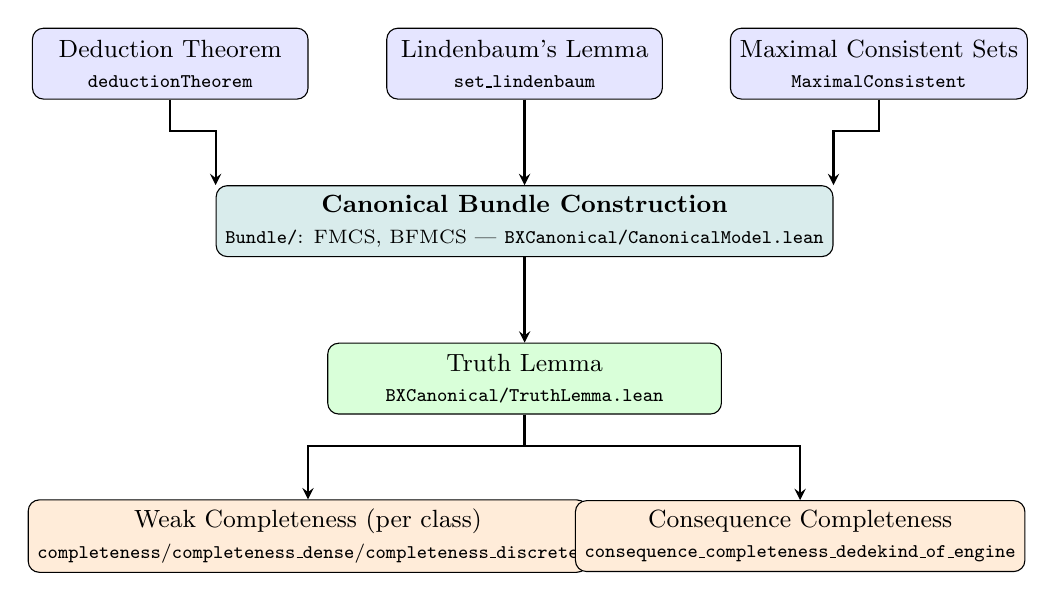
\begin{tikzpicture}[
  box/.style={rectangle, draw, rounded corners, minimum width=3.5cm, minimum height=0.9cm, align=center, font=\small},
  arrow/.style={->, >=stealth, thick}
]
  % Core Infrastructure layer (top) -- Core/
  \node[box, fill=blue!10] (deduct) at (0,6) {Deduction Theorem\\{\scriptsize\texttt{deductionTheorem}}};
  \node[box, fill=blue!10] (linden) at (4.5,6) {Lindenbaum's Lemma\\{\scriptsize\texttt{set\_lindenbaum}}};
  \node[box, fill=blue!10] (mcs) at (9,6) {Maximal Consistent Sets\\{\scriptsize\texttt{MaximalConsistent}}};

  % Canonical-bundle construction layer -- Bundle/ + BXCanonical/CanonicalModel.lean
  \node[box, fill=teal!15, minimum width=6cm] (bundle) at (4.5,4) {\textbf{Canonical Bundle Construction}\\{\scriptsize\texttt{Bundle/}: FMCS, BFMCS\ ---\ \texttt{BXCanonical/CanonicalModel.lean}}};

  % Truth lemma layer
  \node[box, fill=green!15, minimum width=5cm] (truth) at (4.5,2) {Truth Lemma\\{\scriptsize\texttt{BXCanonical/TruthLemma.lean}}};

  % Completeness terminus layer (bottom)
  \node[box, fill=orange!15, minimum width=6.5cm] (weak) at (1.75,0) {Weak Completeness (per class)\\{\scriptsize\texttt{completeness}/\texttt{completeness\_dense}/\texttt{completeness\_discrete}}};
  \node[box, fill=orange!15, minimum width=5cm] (strong) at (8,0) {Consequence Completeness\\{\scriptsize\texttt{consequence\_completeness\_dedekind\_of\_engine}}};

  % Arrows from Core to the canonical-bundle construction
  \draw[arrow] (deduct.south) -- ++(0,-0.4) -| (bundle.north west);
  \draw[arrow] (linden.south) -- (bundle.north);
  \draw[arrow] (mcs.south) -- ++(0,-0.4) -| (bundle.north east);

  % Canonical bundle to Truth Lemma
  \draw[arrow] (bundle.south) -- (truth.north);

  % Truth Lemma to the completeness termini
  \draw[arrow] (truth.south) -- ++(0,-0.4) -| (weak.north);
  \draw[arrow] (truth.south) -- ++(0,-0.4) -| (strong.north);
\end{tikzpicture}
\caption{Dependency structure feeding the landed completeness theorems via the \texttt{BXCanonical} route. \texttt{WeakCanonical.lean} and \texttt{Algebraic.lean} document the other two parallel completeness developments (\S\emph{Three Parallel Completeness Developments} below), which share the \texttt{Core.lean} foundations but not this diagram's \texttt{Bundle.lean}-based construction end-to-end.}
\label{fig:theorem-deps}
\end{figure}

The three foundational components---the \emph{Deduction Theorem}, \emph{Lindenbaum's Lemma}, and \emph{Maximal Consistent Sets}---provide the infrastructure for the canonical bundle construction (\texttt{Bundle/}), which \texttt{BXCanonical/CanonicalModel.lean} uses to build the canonical model.
The truth lemma and the per-class completeness theorems then follow, with the per-class consequence-completeness results following the same pattern via \texttt{StrongCompleteness.lean}.

\subsection{Completeness as Corollary}

The \emph{Completeness Theorems} follow directly from the \emph{Representation Theorem} via contrapositive arguments.

\subsubsection{Weak Completeness}

\begin{theorem}[Weak Completeness]
If $~\satisfies{\varphi}$, then $\proves \varphi$.\footnote{Proven per frame class in \texttt{FormalSystem/Metalogic/BXCanonical/Completeness.lean}: \texttt{completeness} (Base, line 196), \texttt{completeness\_dense} (line 255), and \texttt{completeness\_discrete} (line 296) --- all three \texttt{sorryAx}-free, with axioms exactly \texttt{[propext, Classical.choice, Quot.sound]}. The Dedekind instance \texttt{completeness\_dedekind} is in \texttt{Metalogic/StrongCompleteness.lean}, at the same axiom set.}
\end{theorem}

The proof proceeds by contraposition:
\begin{enumerate}
  \item Assume $\not\proves \varphi$ (i.e., the empty context does not derive $\varphi$).
  \item Then $\{\lneg\varphi\}$ is consistent (otherwise we could derive $\varphi$).
  \item By the \emph{Representation Theorem}, $\{\lneg\varphi\}$ is satisfiable in the canonical model.
  \item So there exists a world where $\lneg\varphi$ is true, meaning $\varphi$ is false.
  \item Hence $\varphi$ is not valid.
\end{enumerate}
By contraposition, validity implies provability.

\subsubsection{Consequence Completeness}

Contexts are finite lists (\texttt{Context = List Formula}), so completeness for consequence
from a context is inter-derivable with weak completeness through the \emph{Deduction Theorem}:
$\context \satisfies \varphi$ iff the iterated implication
$\psi_1 \imp (\psi_2 \imp \cdots (\psi_n \imp \varphi))$ is valid.
We therefore call the arbitrary-context statement \emph{consequence completeness}.
The name \emph{strong completeness} is reserved for the infinite-premise statement discussed in
the next subsection, which is a genuinely different result --- and one that is provably
unavailable for some of the frame classes treated here.

\begin{theorem}[Consequence Completeness]
If $\context \satisfies \varphi$, then $\context \proves \varphi$.\footnote{Landed
\emph{unconditionally} for all four frame classes in
\texttt{FormalSystem/Metalogic/StrongCompleteness.lean}, as
\texttt{consequence\_completeness\_base}, \texttt{consequence\_completeness\_dense},
\texttt{consequence\_completeness\_discrete} and \texttt{consequence\_completeness\_dedekind}.
Each comes with a semantic deduction theorem, a soundness guard
(\texttt{soundness\_base\_consequence} and its dense, discrete and Dedekind siblings) that pins
the consequence relation to the matching soundness theorem and so rules out a vacuous target,
and a weak corollary at $\context = []$. The Dense and Discrete instances are five declarations
each, carrying their own \texttt{SemanticConsequenceDense} / \texttt{SemanticConsequenceDiscrete}
relation; the Base instance is \emph{four}, because it reuses the existing general
\texttt{SemanticConsequence} relation --- for the base class ``all carriers'' \emph{is} the
class, so no restricted relation is needed. The engine-parametric
\texttt{consequence\_completeness\_dedekind\_of\_engine} is retained alongside them as the
pinned interface. All are \texttt{sorryAx}-free at exactly
\texttt{[propext, Classical.choice, Quot.sound]}.}
\end{theorem}

The proof extends weak completeness using an implication chain technique:
\begin{enumerate}
  \item Assume semantic consequence: $\context \satisfies \varphi$.
  \item For context $\context = [\psi_1, \ldots, \psi_n]$, build the implication chain $\psi_1 \imp (\psi_2 \imp \cdots (\psi_n \imp \varphi))$.
  \item Show this chain is valid (from the semantic consequence assumption).
  \item By weak completeness, the chain is provable.
  \item Unfold the chain with repeated modus ponens applications to obtain $\context \proves \varphi$.
\end{enumerate}

Weak completeness is recovered as the $\context = []$ instance, so the weak form has exactly
one proof, as a corollary of the consequence form.

\subsubsection{Strong Completeness and Compactness}

\emph{Strong completeness} proper is completeness for consequence from an arbitrary ---
possibly infinite --- set of premises: $\Gamma \subseteq \mathsf{Form}$, with the finitary
derivability relation $\Gamma \proves \varphi$ iff $\Delta \proves \varphi$ for some finite
$\Delta \subseteq \Gamma$.
Because derivations use only finitely many premises, strong completeness entails compactness of
the semantic consequence relation, so it is available exactly for those frame classes whose
consequence relation is compact.
The classes treated in this development split as follows:

\begin{itemize}
  \item \textbf{Base and Dense}: open --- neither proved nor refuted.
    Neither class imposes Archimedean structure, so no known non-compactness counterexample
    applies; but whether the consequence relation is in fact compact is unsettled.
    A design review of the available routes has been completed and passed, authorising the
    construction sketched below without carrying it out.
    The premise migration to \texttt{Set Formula} is done: \texttt{SetDerivable}, the four per-class
    set consequence relations, and \texttt{Prop}-valued names for each remaining obligation
    (\texttt{CompactBase}, \texttt{ModelExistenceBase}, \texttt{SatisfiableBaseSet},
    \texttt{StrongCompletenessBase} and their Dense siblings) are landed in
    \texttt{Metalogic/SetConsequence.lean}; and
    \texttt{strongCompletenessBase\_of\_compact} / \texttt{strongCompletenessDense\_of\_compact}
    (\texttt{StrongCompleteness.lean}) reduce strong completeness for each class to its compactness
    hypothesis alone --- each deliberately keeping its single-formula \texttt{engine} hypothesis
    live, though that hypothesis is now dischargeable, so that compactness is isolated as
    \emph{the whole} of what remains.
    What is not done is the \emph{model-existence} theorem --- every consistent set of formulas is
    satisfiable in a frame of the class --- which does not follow from the single-formula
    countermodel constructions.
    The recommended route is a bespoke ultraproduct over the finite sublists of $\Gamma$, in four
    steps: an ultraproduct carrier, a \L{}o\'{s} lemma for \texttt{TruthAt}, model existence and
    hence compactness, and finally strong completeness.
    It deliberately abandons the chronicle machinery rather than extending it, and the reason is
    structural rather than a matter of effort: every \texttt{BXCanonical} countermodel routes
    through \texttt{bundleFlow\_completeness\_from\_neg\_membership}
    (\texttt{Algebraic/FlowFrame.lean}), whose three coherence hypotheses are
    relative to a single \texttt{root : Formula} and quantify over \texttt{deferralClosure root},
    with the engine additionally demanding $\varphi \in \texttt{subformulaClosure root}$.
    Both closures are \texttt{Finset}-valued, whereas an infinite $\Gamma$ would need coherence over
    $\bigcup_{\psi \in \Gamma} \texttt{subformulaClosure}\;\psi$, which is not a \texttt{Finset} and
    has no single root to be relative to.
    The set-level consistency layer (\texttt{SetConsistent}, \texttt{SetMaximalConsistent},
    \texttt{set\_lindenbaum} in \texttt{FormalSystem/Metalogic/Core/MaximalConsistent.lean}) is
    already finitary and in place.
  \item \textbf{Discrete}: provably unavailable --- and this is a theorem, not a remark.
    \texttt{discrete\_consequence\_not\_compact} refutes \texttt{CompactDiscrete} and
    \texttt{strongCompletenessDiscrete\_refuted} refutes \texttt{StrongCompletenessDiscrete}
    outright, both in \texttt{Metalogic/DiscreteNonCompactness.lean} and both
    \texttt{sorryAx}-free at exactly \texttt{[propext, Classical.choice, Quot.sound]} under the
    \texttt{\#print axioms} audit block at the end of that file.
    The witness is \texttt{archWitness}: on discrete orders the next-step operator
    $X\varphi = U(\varphi, \bot)$ is genuine, so the premise set
    $\{F p\} \cup \{\lneg X^n p : n \in \mathbb{N}\}$ is expressible, and its two halves are
    \texttt{archWitness\_finitely\_satisfiable} (finite satisfiability over $\mathbb{Z}$, placing
    $p$ far enough out) and \texttt{archWitness\_not\_satisfiable} (unsatisfiability over every
    Archimedean discrete order, since the $F p$ witness would lie at some finite successor
    distance).
    The consequence relation is therefore not compact, and weak completeness --- with its
    finite-context consequence corollary \texttt{consequence\_completeness\_discrete} --- is the
    strongest form for this class.
  \item \textbf{Dedekind}: unavailable on the primary source's own terms --- a weaker claim
    than Discrete's, and one that must not be read as sharing its status.
    Completeness over real-flowed (Dedekind complete) time is \emph{weak} in Reynolds' sense
    (Reynolds 1992, Theorem 7), and the restriction there is genuine rather than an artefact of
    presentation.
    What this development does \emph{not} contain is a refutation: there is no
    \texttt{CompactDedekind} definition and no refuting theorem anywhere in the tree, so for this
    class the infinitary statement is \emph{unproved} rather than settled negatively.
    Weak completeness, with its finite-context consequence corollary
    \texttt{consequence\_completeness\_dedekind}, is the strongest form established here.
\end{itemize}

\paragraph{Provable iff Valid.}
No unconditional $\proves \varphi \iff \satisfies{\varphi}$ declaration exists under a single name.
The biconditional holds compositionally per frame class: the right-to-left direction is \texttt{completeness}/\texttt{completeness\_dense}/\texttt{completeness\_discrete} (\texttt{FormalSystem/Metalogic/BXCanonical/Completeness.lean}), and the left-to-right direction is \texttt{soundness}/\texttt{soundness\_dense}/\texttt{soundness\_discrete} (\texttt{FormalSystem/Metalogic/Soundness.lean}).

This biconditional shows that the proof system and semantics align perfectly.
Soundness (left-to-right) ensures no non-logical consequences are derivable, while completeness (right-to-left) ensures all logical consequences are captured by the proof system.
Together, they establish that \textbf{TM} provides an exact syntactic characterization of semantic validity, per frame class.

\subsubsection{Three Parallel Completeness Developments}

The codebase's completeness proof is not a single syntactic-versus-semantic dichotomy.
It has three independently-developed, parallel completeness routes sharing common foundations.

\paragraph{Shared foundation (\texttt{Core/}).}
\texttt{Consistent}, \texttt{MaximalConsistent}, \texttt{SetConsistent}, \texttt{SetMaximalConsistent}, \texttt{set\_lindenbaum}, \texttt{contextToSet}, and \texttt{deductionTheorem}/\texttt{Derivable.deduction} are shared by all three routes below; none is tied to any one of them.

\paragraph{\texttt{BXCanonical/} --- the BX (chronicle/Henkin-style) route.}
Builds a \texttt{BFMCS Int} via the chain construction described above and is the home of the landed \texttt{completeness}/\texttt{completeness\_dense}/\texttt{completeness\_discrete} theorems.

\paragraph{\texttt{WeakCanonical/} --- the Reynolds/Doets discrete route.}
Includes the large \texttt{Kamp/} subtree (Kamp's-theorem-style normal-form translation machinery bridging temporal formulas to monadic first-order structures for the Doets $k$-types argument).
Its export \texttt{countermodel\_discrete} (\texttt{WeakCanonical/Transfer.lean}) is the \emph{deprecated} fallback still wired into the general \texttt{completeness} theorem's discrete branch, and is the sole sorry source (see \emph{Implementation Status} below); its sorry-free sibling \texttt{countermodel\_discrete\_reynolds\_v2} (\texttt{WeakCanonical/IntegerModel/ReynoldsBridge.lean:739}) is what \texttt{completeness\_discrete} actually uses.
These are two different pipelines and must not be conflated.

\paragraph{\texttt{Algebraic/} --- the Lindenbaum-Tarski quotient-algebra route.}
\texttt{LindenbaumQuotient.lean}, \texttt{ParametricCanonical.lean}, \texttt{ParametricTruthLemma.lean}, \texttt{UltrafilterMCS.lean}.
Closest in spirit to the archived syntactic approach's quotient-flavored construction below, but a \emph{third}, independently-developed route, not the same construction under a new name, and not currently the route feeding the landed \texttt{completeness*} theorems.

\texttt{Bundle/} supplies the shared canonical-frame vocabulary (\texttt{FMCS}, \texttt{BFMCS}) used by \texttt{BXCanonical/}.
None of the three routes above is claimed to be primary beyond the verifiable fact that \texttt{BXCanonical/} is where the landed completeness theorems live.

% TODO (carried forward, restated against the live construction): the archived syntactic
% approach below is in the correct spirit and should be ported over from the Boneyard for
% careful study and full implementation. By contrast, none of the three live routes above
% builds a semantic object directly out of pure syntax the way the syntactic approach does.

\paragraph{Archived: Syntactic Approach.}
World states were directly identified with maximal consistent sets, with accessibility defined via modal witnesses: $\nec\varphi \in w$ implies $\varphi \in w'$ for all accessible $w'$.
This approach required explicit negation-completeness proofs for locally consistent sets and is archived in \texttt{Boneyard/} for historical reference; it is not one of the three current developments above, and its archival is a matter of historical record rather than a claim that the live routes supersede it in spirit.

\subsection{Decidability}

The decidability of TM bimodal logic rests on the \emph{Finite Model Property}: if a formula is satisfiable, it is satisfiable in a finite model bounded by the formula's modal and temporal depth.
The bound on model size is $2^{|\mathsf{closure}(\varphi)|}$, where the subformula closure contains all relevant formulas for determining the truth of $\varphi$.
This bound is proved, not conjectural: \texttt{filtered\_world\_bound} establishes $\mathsf{Nat.card}\,(\mathsf{FilteredWorld}\,\varphi) \leq 2^{|\mathsf{closure}(\varphi)|}$, and \texttt{assignmentSpace\_card} computes the right-hand side as an equality: the space of truth assignments to the subformula closure has exactly $2^{|\mathsf{closure}(\varphi)|}$ elements.
Both are obtained from the injectivity of the characteristic-set map on filtered worlds (\texttt{filteredCharacteristicSet\_injective}), which is also what witnesses finiteness.
This property connects the representation infrastructure to decidability by ensuring that satisfiability checking can terminate.

The decidability proof proceeds via a tableau-based decision procedure.

\begin{remark}[Decidability is not yet a theorem here]
An earlier version of this section stated, as a theorem, that validity in TM bimodal logic is decidable, on the ground that for any formula $\varphi$ either $\valid{\varphi}$ or $\neg\valid{\varphi}$.
That statement is a consequence of excluded middle for an arbitrary proposition and carries no decidability content: it holds of every predicate whatsoever, produces no procedure, and yields no \texttt{Decidable} instance.
The two Lean theorems it corresponded to were correspondingly vacuous and have been deleted.

What is proved is the semantic soundness of the tableau calculus: every rule the procedure can schedule at a given frame class preserves satisfiability under that class's carrier property, for all $34$ rules and all four frame classes (\texttt{ruleSound\_of\_mem\_allRulesForFC}).
Constructive decidability of validity additionally requires the equivalence between a formula's validity and the closure of every tableau branch, together with the termination bound and the truth-lemma gate, and obligations for the two rules scheduled outside the frame-class rule set.
That remains open.
\end{remark}

\begin{theorem}[Decision Soundness]
If the decision procedure returns ``valid'' with proof $\pi$, then $\valid{\varphi}$.\footnote{This is proven as \texttt{decide\_sound}.}
\end{theorem}

Here $\pi$ is a derivation term witnessing $\proves \varphi$, constructed from the closed tableau.
In Lean 4, this is a term of type \texttt{Derivable FrameClass.Base [] $\varphi$}, representing a formal proof tree.

The decision procedure operates as follows:
\begin{enumerate}
  \item \textbf{Direct axiom proof}: Check if $\varphi$ matches one of the axiom schemata directly, yielding an immediate derivation.
  \item \textbf{Proof search}: Apply Lean 4 tactics (\texttt{decide}, \texttt{simp}) with bounded recursion depth to find a derivation automatically.
  \item \textbf{Tableau construction}: Build a systematic tree that decomposes $\varphi$ into simpler signed formulas.
  \item If all branches close: formula is valid, extract proof.
  \item If open saturated branch: formula is invalid, extract countermodel.
\end{enumerate}

A \emph{tableau} is a tree-structured refutation method: to prove $\varphi$ valid, we assume $\varphi$ is false and systematically derive contradictions.
Each branch represents a possible scenario; if all branches lead to contradictions, the original assumption was impossible, so $\varphi$ must be valid.

\subsubsection{Tableau Structure}

The tableau uses \textbf{signed formulas} with annotations:
\begin{itemize}
  \item $T(\varphi)$: formula $\varphi$ is assumed true
  \item $F(\varphi)$: formula $\varphi$ is assumed false
\end{itemize}

\textbf{Expansion rules} are categorized as:
\begin{itemize}
  \item \textbf{Propositional}: $T(\varphi \land \psi)$ splits, $F(\varphi \imp \psi)$ splits, etc.
  \item \textbf{Modal}: $T(\nec\varphi)$ propagates to accessible worlds, $F(\poss\varphi)$ creates witness
  \item \textbf{Temporal}: $T(\always\varphi)$ propagates to future times, $F(\sometimes\varphi)$ creates witness
\end{itemize}

\noindent
A branch \textbf{closes} when it contains both $T(\varphi)$ and $F(\varphi)$ for some formula.
A branch is \textbf{saturated} when no expansion rules apply.

\subsubsection{Complexity}

\begin{center}
\begin{tabular}{@{}ll@{}}
\toprule
Measure & Complexity \\
\midrule
Time & $O(2^n)$ where $n$ is formula size \\
Space & $O(n)$ \\
Class & PSPACE-complete \\
\bottomrule
\end{tabular}
\end{center}

The exponential time bound means formulas of modest size (30--50 symbols) remain tractable on modern hardware.
PSPACE-completeness implies that modal satisfiability is among the hardest problems solvable with polynomial space, but the linear space bound makes memory usage manageable even for larger formulas.

% TODO: it would also help to explain where the calculations come from (how these numbers are calculated) and check that they are in fact correct as stated

\subsubsection{Decision Result Types}

The decision procedure returns one of three outcomes:
\begin{itemize}
  \item \texttt{valid proof}: Formula is valid with derivation tree
  \item \texttt{invalid counter}: Formula is invalid with countermodel
  \item \texttt{timeout}: Resources exhausted before decision
\end{itemize}

Despite computational limitations, decidability is practically valuable: small formulas (most proof obligations in practice) resolve quickly, invalid formulas are often rejected early without full exploration, and countermodels provide concrete feedback for debugging specifications.

\subsection{File Organization and Dependencies}

The active metalogic infrastructure is in \texttt{FormalSystem/Metalogic/}, organized as a shared \texttt{Core/} foundation beneath three parallel completeness developments (\texttt{BXCanonical/}, \texttt{WeakCanonical/}, \texttt{Algebraic/}) plus the shared \texttt{Bundle/} canonical-frame construction (\S\emph{Three Parallel Completeness Developments} above), alongside \texttt{Soundness.lean}, \texttt{StrongCompleteness.lean}, and \texttt{Decidability/}.
The following diagram illustrates this top-level layout at summary level; \texttt{WeakCanonical/Kamp/} (approximately 90 files) and \texttt{Decidability/Verified/} are large internal machinery, named here but not expanded.

\begin{center}
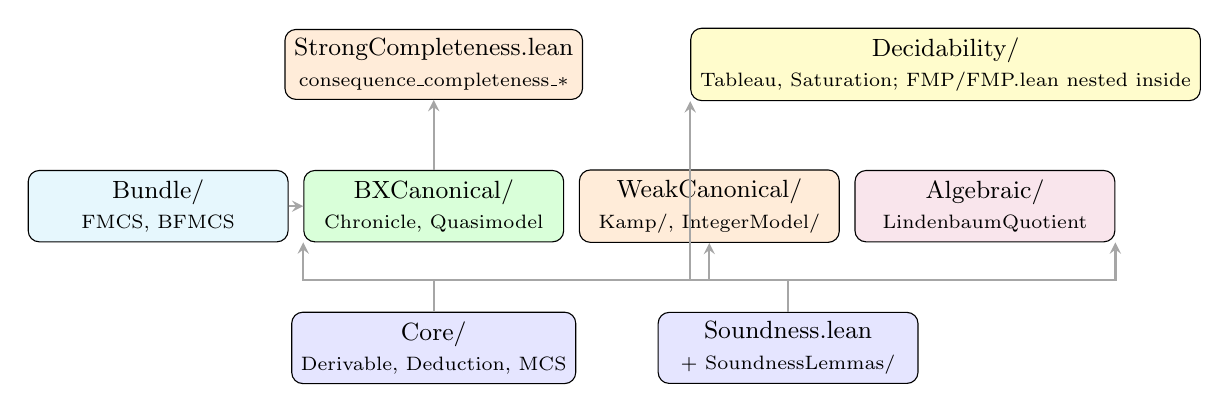
\begin{tikzpicture}[
  dirbox/.style={rectangle, draw, rounded corners, minimum width=3.3cm, minimum height=0.7cm, align=center, font=\small},
  arrow/.style={->, >=stealth, thick, gray!70}
]
  % Core layer (bottom)
  \node[dirbox, fill=blue!10] (core) at (1.5,0) {Core/\\{\scriptsize Derivable, Deduction, MCS}};
  \node[dirbox, fill=blue!10] (sound) at (6,0) {Soundness.lean\\{\scriptsize + SoundnessLemmas/}};

  % Bundle and the three parallel completeness routes
  \node[dirbox, fill=cyan!10] (bundle) at (-2,1.8) {Bundle/\\{\scriptsize FMCS, BFMCS}};
  \node[dirbox, fill=green!15] (bx) at (1.5,1.8) {BXCanonical/\\{\scriptsize Chronicle, Quasimodel}};
  \node[dirbox, fill=orange!15] (weak) at (5,1.8) {WeakCanonical/\\{\scriptsize Kamp/, IntegerModel/}};
  \node[dirbox, fill=purple!10] (alg) at (8.5,1.8) {Algebraic/\\{\scriptsize LindenbaumQuotient}};

  % Consequence completeness and decidability
  \node[dirbox, fill=orange!15] (strong) at (1.5,3.6) {StrongCompleteness.lean\\{\scriptsize consequence\_completeness\_$\ast$}};
  \node[dirbox, fill=yellow!20, minimum width=4cm] (decid) at (8,3.6) {Decidability/\\{\scriptsize Tableau, Saturation; FMP/FMP.lean nested inside}};

  % Arrows
  \draw[arrow] (bundle.east) -- (bx.west);
  \draw[arrow] (core.north) -- ++(0,0.4) -| (bx.south west);
  \draw[arrow] (core.north) -- ++(0,0.4) -| (weak.south);
  \draw[arrow] (core.north) -- ++(0,0.4) -| (alg.south east);
  \draw[arrow] (bx.north) -- (strong.south);
  \draw[arrow] (sound.north) -- ++(0,0.4) -| (decid.south west);
\end{tikzpicture}
\end{center}

\noindent
\textbf{Directory descriptions}:
\begin{itemize}
  \item \textbf{\texttt{Core/}}: Shared foundational definitions -- provability (\texttt{Derivable}), the deduction theorem, and maximal consistent sets (\texttt{Consistent}, \texttt{MaximalConsistent}, \texttt{set\_lindenbaum}).
  \item \textbf{\texttt{Bundle/}}: Shared canonical-frame construction (\texttt{FMCS}, \texttt{BFMCS}) used by \texttt{BXCanonical/}.
  \item \textbf{\texttt{BXCanonical/}}: The BX (chronicle/Henkin-style) completeness route; home of the landed \texttt{completeness}/\texttt{completeness\_dense}/\texttt{completeness\_discrete} theorems.
  \item \textbf{\texttt{WeakCanonical/}}: The Reynolds/Doets discrete completeness route, including the large \texttt{Kamp/} subtree.
  \item \textbf{\texttt{Algebraic/}}: The Lindenbaum-Tarski quotient-algebra completeness route.
  \item \textbf{\texttt{Soundness.lean} (+ \texttt{SoundnessLemmas/})}: Validity proofs for all 15 axiom schemata and the main soundness theorems.
  \item \textbf{\texttt{StrongCompleteness.lean}}: The per-class finite-context consequence-completeness layer, unconditional for all four frame classes, plus the two compactness reductions \texttt{strongCompleteness\{Base,Dense\}\_of\_compact}; the engine-parametric \texttt{consequence\_completeness\_dedekind\_of\_engine} is retained as the pinned interface.
\item \textbf{\texttt{SetConsequence.lean}}: The \texttt{Set Formula} vocabulary the strong-completeness statements are phrased in --- \texttt{SetDerivable}, the four per-class set consequence relations, and \texttt{Prop}-valued names for the open Base/Dense obligations and the refuted Discrete ones.
\item \textbf{\texttt{DiscreteNonCompactness.lean}}: The machine-checked refutations \texttt{discrete\_consequence\_not\_compact} and \texttt{strongCompletenessDiscrete\_refuted}, via the \texttt{archWitness} premise set.
  \item \textbf{\texttt{Decidability/}}: Tableau-based decision procedure with proof/countermodel extraction; the finite model property lives nested inside at \texttt{Decidability/FMP/FMP.lean}, not as a top-level hub.
\end{itemize}

\subsection{Implementation Status}

\subsubsection{Sorry Status}

The live per-class completeness picture, in \texttt{FormalSystem/Metalogic/BXCanonical/Completeness.lean} unless noted:

\begin{itemize}
  \item \texttt{completeness} (Base, line 196), \texttt{completeness\_dense} (line 255) and \texttt{completeness\_discrete} (line 296) are all \textbf{\texttt{sorryAx}-free}, with axioms exactly \texttt{[propext, Classical.choice, Quot.sound]}. The Base instance's discrete branch no longer routes through the deprecated \texttt{WeakCanonical.countermodel\_discrete} fallback: it is proved at the non-Archimedean discrete carrier $\mathbb{Q} \times_{\ell} \mathbb{Z}$ in \texttt{WeakCanonical/GroupModel/CountermodelBase.lean}, off \texttt{companionChronicle}.
\item \texttt{completeness\_dedekind} and \texttt{consequence\_completeness\_dedekind} are landed \textbf{unconditionally} in \texttt{Metalogic/StrongCompleteness.lean}, at the same axiom set, with \texttt{\#print axioms} audits in that file; the engine hypothesis is discharged by \texttt{BXCanonical.completeness\_dedekind\_engine}. The engine-parametric \texttt{completeness\_dedekind\_of\_engine} and \texttt{consequence\_completeness\_dedekind\_of\_engine} are retained unmodified alongside them as the pinned interface.
\item The per-class finite-context consequence layer --- \texttt{consequence\_completeness\_base}, \texttt{\ldots\_dense}, \texttt{\ldots\_discrete}, \texttt{\ldots\_dedekind}, each with its soundness guard and weak corollary --- is likewise \texttt{sorryAx}-free at the same axiom set, audited in \texttt{StrongCompleteness.lean}.
\end{itemize}

\noindent
No live \texttt{sorryAx} remains on any of these paths. The \texttt{succ\_cofinal} argument behind the former \texttt{WeakCanonical.countermodel\_discrete} fallback was characterized as provably unfixable and has been archived; the Base-frame discrete branch was closed by a genuine new construction at $\mathbb{Q} \times_{\ell} \mathbb{Z}$ rather than by re-wiring that fallback.

\subsubsection{Decidability Implementation}

\begin{center}
\begin{tabular}{@{}lll@{}}
\toprule
Submodule & Status & Notes \\
\midrule
SignedFormula & Complete & Sign, SignedFormula, Branch types \\
Tableau & Complete & Expansion rules \\
Closure & Complete & Branch closure detection \\
Saturation & Complete & Fuel-based termination \\
ProofExtraction & Partial & Axiom instances only \\
CountermodelExtraction & Complete & From open branches \\
DecisionProcedure & Complete & Main decide function \\
Soundness & Proven & \texttt{decide\_sound} \\
Completeness & Partial & Requires Finite Model Property \\
\bottomrule
\end{tabular}
\end{center}

\subsubsection{Metalogic Implementation}

\begin{center}
\begin{tabular}{@{}lll@{}}
\toprule
Component & Status & Lean \\
\midrule
Soundness & Proven & \texttt{soundness} \\
Deduction Theorem & Proven & \texttt{deductionTheorem} (general form: \texttt{Derivable.deduction}) \\
Lindenbaum Lemma & Proven & \texttt{set\_lindenbaum} \\
Canonical Bundle & Proven & \texttt{FMCS}, \texttt{BFMCS} (\texttt{Bundle/}) \\
Truth Lemma & Proven (per development) & \texttt{BXCanonical/TruthLemma.lean} \\
Weak Completeness & Proven* & \texttt{completeness}/\texttt{completeness\_dense}/\texttt{completeness\_discrete} \\
Consequence Completeness & Proven, all four classes & \texttt{consequence\_completeness\_\{base,dense,discrete,dedekind\}} \\
Strong Completeness & Reduced to compactness & \texttt{strongCompleteness\{Base,Dense\}\_of\_compact} \\
Finite Model Property & Statement & \texttt{mcs\_finite\_model\_property} \\
Decidability Soundness & Proven & \texttt{decide\_sound} \\
\bottomrule
\end{tabular}
\end{center}

\noindent
* Weak completeness is proven for all four frame classes ---
\texttt{completeness}, \texttt{completeness\_dense}, \texttt{completeness\_discrete} and
\texttt{completeness\_dedekind} --- and every one of them is \texttt{sorryAx}-free at exactly
\texttt{[propext, Classical.choice, Quot.sound]}.
Consequence completeness is likewise unconditional for all four classes, at the same axiom set;
the engine-parametric \texttt{\ldots\_of\_engine} forms are retained as pinned interfaces rather
than as the only landed statements.
These are \emph{finite}-context results (\texttt{Context = List Formula}) and are therefore not
strong completeness.
Genuine strong completeness over infinite premise sets is a separate statement with three
distinct statuses across the classes: machine-refuted for Discrete, open for Base and Dense
(each reduced to its compactness hypothesis by
\texttt{strongCompleteness\{Base,Dense\}\_of\_compact}), and unavailable on Reynolds' own terms
--- unproved, not refuted --- for Dedekind.
See \emph{Strong Completeness and Compactness}.

\end{document}
